\chapter{Scores}\label{chap:scoring}
Möchten wir mehrere verschiedene Vorhersagen miteinander vergleichen, so ist es naheliegend, jeder Vorhersage einen einzelnen Wert zuzuordnen, der sowohl die Kalibrierung als auch die Schärfe berücksichtigt. Anhand diesen Wertes ließe sich die Qualität der Vorhersagen vergleichen und diejenige mit dem besten Wert auswählen. Dafür können wir Scores verwenden. Hierbei verwenden wir die Konvention, Scores als Verlustfunktionen zu betrachten, sodass kleinere Scores eine bessere Vorhersagegüte bedeuten. 

In Abschnitt \ref{seq:score_propertiers} definieren wir Scores und ihre Eigenschaften. Anschließend betrachten wir in Abschnitt \ref{seq:crps_qs} zwei etabilierte Scores und wie sie zusammenhängen: Den Quantilscore und den \TCRPS \;(CRPS).

Dazu bleiben wir im Vorhersageraumsetting $(F,Y)$. Zusätzlich sei $\mathcal F$ eine Familie von Wahrscheinlichkeitsverteilungen auf $\mathbb R$ mit existierendem und endlichem Erwartungswert. Sowohl die möglichen Vorhersageverteilungen als auch die bedingten Verteilungen von $Y$ bezüglich der Information $\sigma(F)$ sollen (fast sicher) in dieser Familie $\mathcal F$ liegen. Weiter nehmen wir an, dass alle auftretenden Erwartungswerte existieren und endlich sind. Wahrscheinlichkeitsverteilungen identifizieren wir mit ihren Verteilungsfunktionen. Schließlich  bezeichnen wir mit $\overline{\mathbb R}$ die erweiterten reellen Zahlen.

\section{Grundlagen und Eigenschaften} \label{seq:score_propertiers}
Je nach Anwendungsfall kann eine Vorhersage verschiedene Formen annehmen: Sie kann eine vollständige probabilistische Vorhersage sein, aber auch ein einzelner reeller Wert, etwa ein Quantil oder ein Erwartungswert. Um beide Fälle einheitlich behandeln zu können, bezeichnen wir mit $\mathcal{V}$ die Menge der möglicher Vorhersagen eines Typs. Abhängig vom Kontext gilt dann entweder $\mathcal{V} = \mathcal{F}$ oder $\mathcal{V} = \mathbb{R}$.

\begin{defi}[Score \parencite{gneitingMakingPoint2011}]
Sei $\mathcal V$ eine Menge aus einzelnen Vorhersagen. Eine Funktion
\[
S:\mathcal V\times\mathbb R\to\overline{\mathbb R},\quad (v,y)\mapsto S(v,y),
\]
heißt \emph{Scoring-Rule} bzw. \emph{Scoring-Function} oder einfach \emph{Score}, wenn sie ein Vorhersage-Beobachtungspaar $(v,y)$ auf eine Zahl abbildet.

Die obige Definition ist bewusst allgemein gehalten. Abhängig von der Art der Vorhersage $\mathcal V$ ergeben sich zwei Spezialisierungen:
\begin{itemize}
    \item $\mathcal{V}=\F$: Hierbei handelt es sich um Scoring-Rules. Es sind Scores für probabilistische Vorhersagen, bei denen vollständige Wahrscheinlichkeitsverteilungen bewertet werden. Die zentrale Eigenschaft solcher Scoring-Rules ist die \emph{Properness}.
    \item $\mathcal V=\R$: In diesem Fall entsprechen die Vorhersagen reellwertigen Punktprognosen oder statistischen Funktionalen von probabilistischen Vorhersagen. Wir nennen diese Scores; Scoring-Functions. Die zentrale Eigenschaft solcher Scoring-Functions ist die \emph{Konsistenz}. Für diese Arbeit beschränken wir uns auf Scoring-Functions für Quantile.\\
\end{itemize}
\end{defi}


\noindent
Zum Bewerten und Vergleichen von Vorhersagen bestimmen wir den erwarteten Score \parencite{gneiting2014probabilistic}.
\begin{defi}[Erwarteter Score]\label{def:exp_score}
Sei $(F,Y)$ ein Vorhersageraum und $S$ ein Score
Wir definieren den \emph{erwarteten Score} durch
\[
\bar S \coloneqq \E_\PW[S(V,Y)],
\]
wobei $V$ die jeweilige Vorhersage bezeichnet: Im Fall $\mathcal{V} = \mathcal{F}$  gilt $V = F$, im Fall $\mathcal{V} = \mathbb{R}$ gilt $V = \qF$ für ein  $\alpha$-Quantil der Verteilung $F$.
\end{defi}{}

Empirisch bestimmen wir den erwarteten Score als mittleren Score über alle Vorhersage-Beobachtungspaare, die wir betrachten \parencite{gneiting2014probabilistic}.
\begin{defi}[Empirisch erwarteter Score oder mittlerer Score]\label{def:emp_exp_score}
Für eine Stichprobe von Vorhersage-Beobachtungspaaren
$(v_i,y_i)$, $i=1,\dotsc,n$ ergibt sich der \emph{empirische erwartete Score} oder \emph{mittlerer Score}  als
\[
\hat S\coloneqq \frac1n\sum_{i=1}^n S(v_i,y_i),
\]
wobei wir je nach Art des Scores $S$ Vorhersage-Beobachtungspaare der Form \ref{eq:stich} oder \ref{eq:qaunt_stich_emp} betrachten.
\end{defi}{}
\noindent
Dieser Kennwert stellt das entscheidenende praktische Bewertungsmaß einer Vorhersage dar. Es folgen die zentralen Eigenschaften von Scores: \emph{Properness} und \emph{Konsistenz}.
\begin{defi}[Proper Score \texorpdfstring{\parencite[Definition 4]{gneiting2014probabilistic}})]
Eine Score der Form 
\[S: \F \times \R \to \overline{\R},\quad (P,y) \mapsto S(P,y)\] heißt proper relativ zu $\F$, falls für alle $P,Q \in \F$
\[
\E_{Y\sim Q}[S(Q,Y)]\leq \E_{Y\sim Q}[S(P,Y)]
\]
gilt.
\end{defi}

Properness bedeutet also, dass es im Erwartungswert optimal ist, die tatsächliche Wahrscheinlichkeitsverteilung des Vorhersagegegenstandes vorherzusagen. Jede davon abweichende Vorhersage führt zu einem mindestens ebenso großen erwarteten Score.

Hingegen ist die Konsistenz eines Scores eine Eigenschaft im Zusammenhang mit statistischen Funktionalen, etwa dem Erwartungswert, Schwellenwerten oder Quantilen \parencite[Definition 5]{gneiting2014probabilistic}. Wir beschränken uns weiterhin auf Quantile.

%mini anpassung
\begin{defi}[$\alpha$-Quantil konsistenter Score]
\label{def::consistent}
Eine Score der Form \[S: \mathbb{R} \times \mathbb{R} \to \overline{\mathbb{R}},\quad (x,y) \mapsto S(x,y)\] heißt konsistent bzgl. des $\alpha$-Quantils relativ zu $\F$, falls für alle $x \in \R$ und $Q \in \F$ 
\[
\E_{Y\sim Q}[S(q_\alpha(Q),Y)]\leq \E_{Y\sim Q}[S(x,Y)]\quad 
\]
gilt.
\end{defi}
Eine $\alpha$-quantil konsistenter Score ist somit so konstruiert, dass im Erwartungswert das wahre (bedingte) $\alpha$-Quantil optimal ist.

Die beiden Arten von Scores lassen sich ineinander überführen. So induziert ein konsistenter Score stets einen proper Score \parencite[Theorem 3]{gneitingMakingPoint2011}. Gleichzeitig zeigt sich daran, dass Properness allein als Eigenschaft nicht hinreichend für einen guten Score ist, wie im Appendix \ref{chap:other_examp} an Beispiel \ref{bsp:propernogood} deutlich wird. Daher ist es sinnvoll, auf etablierte Scores zurückzugreifen.

Im Folgenden betrachten wir zwei solcher etablierter Scores: Den \emph{Quantilscore} als $\alpha$-Quantil konsistenten Score und den \emph{\TCRPS} (CRPS) als proper Score. Dabei handelt es sich um Scores, die beide einen Minimalwert von null haben.

\section{Quantilscore und \TCRPS} \label{seq:crps_qs}
Die folgenden Scores betrachten wir relativ zur Klasse der Wahrscheinlichkeitsmaße auf $\R$ mit existierendem und endlichem Erwartungswert.

Ein konsistenter Score für das $\alpha$-Quantil ist der Quantilscore (auch Pinball Loss) \parencite[Theorem 9 (c)]{gneitingMakingPoint2011}. Er lautet
\[
\QS_\alpha(x,y) = \left(\mathds{1}\{y\le x\} - \alpha \right)(x-y)
\]
oder ausgeschrieben
\[
\QS_\alpha(x,y)=\begin{cases}
(1-\alpha)(x-y), & \text{falls } y \le x,\\[0.5em]
\alpha(y-x), & \text{falls } y > x.
\end{cases}
\]
Abhängig des gewählten $\alpha$-Quantils gewichtet der Score die Differenz $(x-y)$ zwischen beobachtetem Wert $x$ und vorhergesagtem Quantil $y$  unterschiedlich. Beim Median ist der Score symmetrisch, sodass Über- und Unterschätzungen gleich gewichtet werden. Liegt das Quantil über dem Median, werden zu niedrige Vorhersagen stärker bestraft. Liegt es unter dem Median, werden zu hohe Vorhersagen stärker bestraft. Abbildung \ref{fig:qs_visu} zeigt den Quantilscore abhängig der Differenz $(x-y)$ für das $25\%,50\%,75\%$ Quantil.


\begin{figure}[!h]
    \centering
    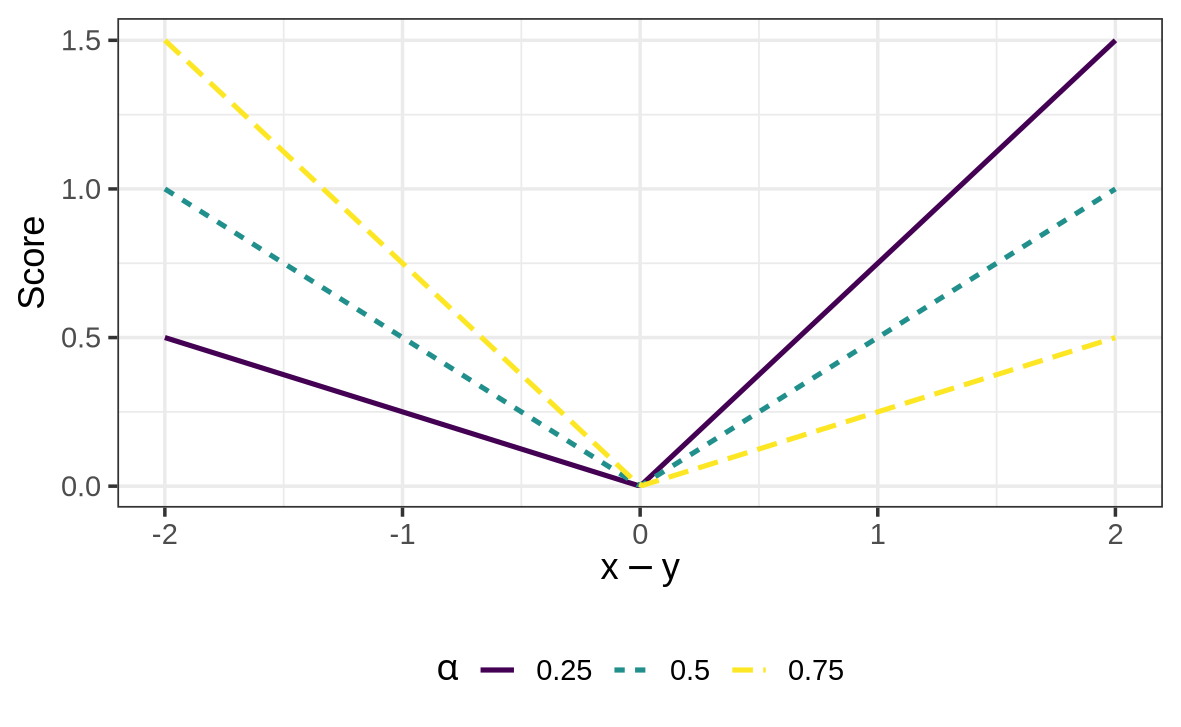
\includegraphics[width=0.75\linewidth]{figs/qs_visu_Rplot.png}
    \caption{Quantilscore abhängig der Differenz $(x-y)$ für das $25\%,50\%,75\%$ Quantil.}
    \label{fig:qs_visu}
\end{figure}

Schließlich bestimmen wir für Vorhersage-Beobachtungspaare der Form \eqref{eq:stich}  den empirischen Gesamtscore entsprechend Definition \ref{def:emp_exp_score} als
\[
\widehat{\QS}_\alpha = \frac{1}{n}\sum_{i=1}^{n}\QS_\alpha\big(q_\alpha(F_i),y_i\big).
\]
Die Höhe der erwarteten Quantilscores hängt ebenfalls vom gewählten Quantilniveau ab. Häufig werden für mittlere Quantile größere erwartete Quantilscores beobachtet als für Randquantile. Ein Grund ist jene asymmetrische Gewichtung des Quantilscores, durch die bei Randquantilen jeweils eine Fehlerseite nur gering gewichtet wird. Liegen die Vorhersagefehler überwiegend auf dieser Seite, tragen sie entsprechend nur wenig zum Quantilscore bei. Der genaue Verlauf des erwarteten Quantilscores hängt jedoch von der zugrundeliegenden Vorhersage ab.


Als nächstes führen wir den \emph{\TCRPS}$\;$(CRPS) als einen proper Score ein. Er lautet
\[
\CRPS(F,y)=\int_\R \left(F(x)-\mathds{1}\{y\leq x\}\right)^2 \,dx
\]
\parencite{Gneiting2007}. Abbildung \ref{fig:crps_visu} verdeutlicht eine geometrische Interpretation des CRPS für beispielhafte Vorhersagen.

\begin{figure}[!h]
    \centering
    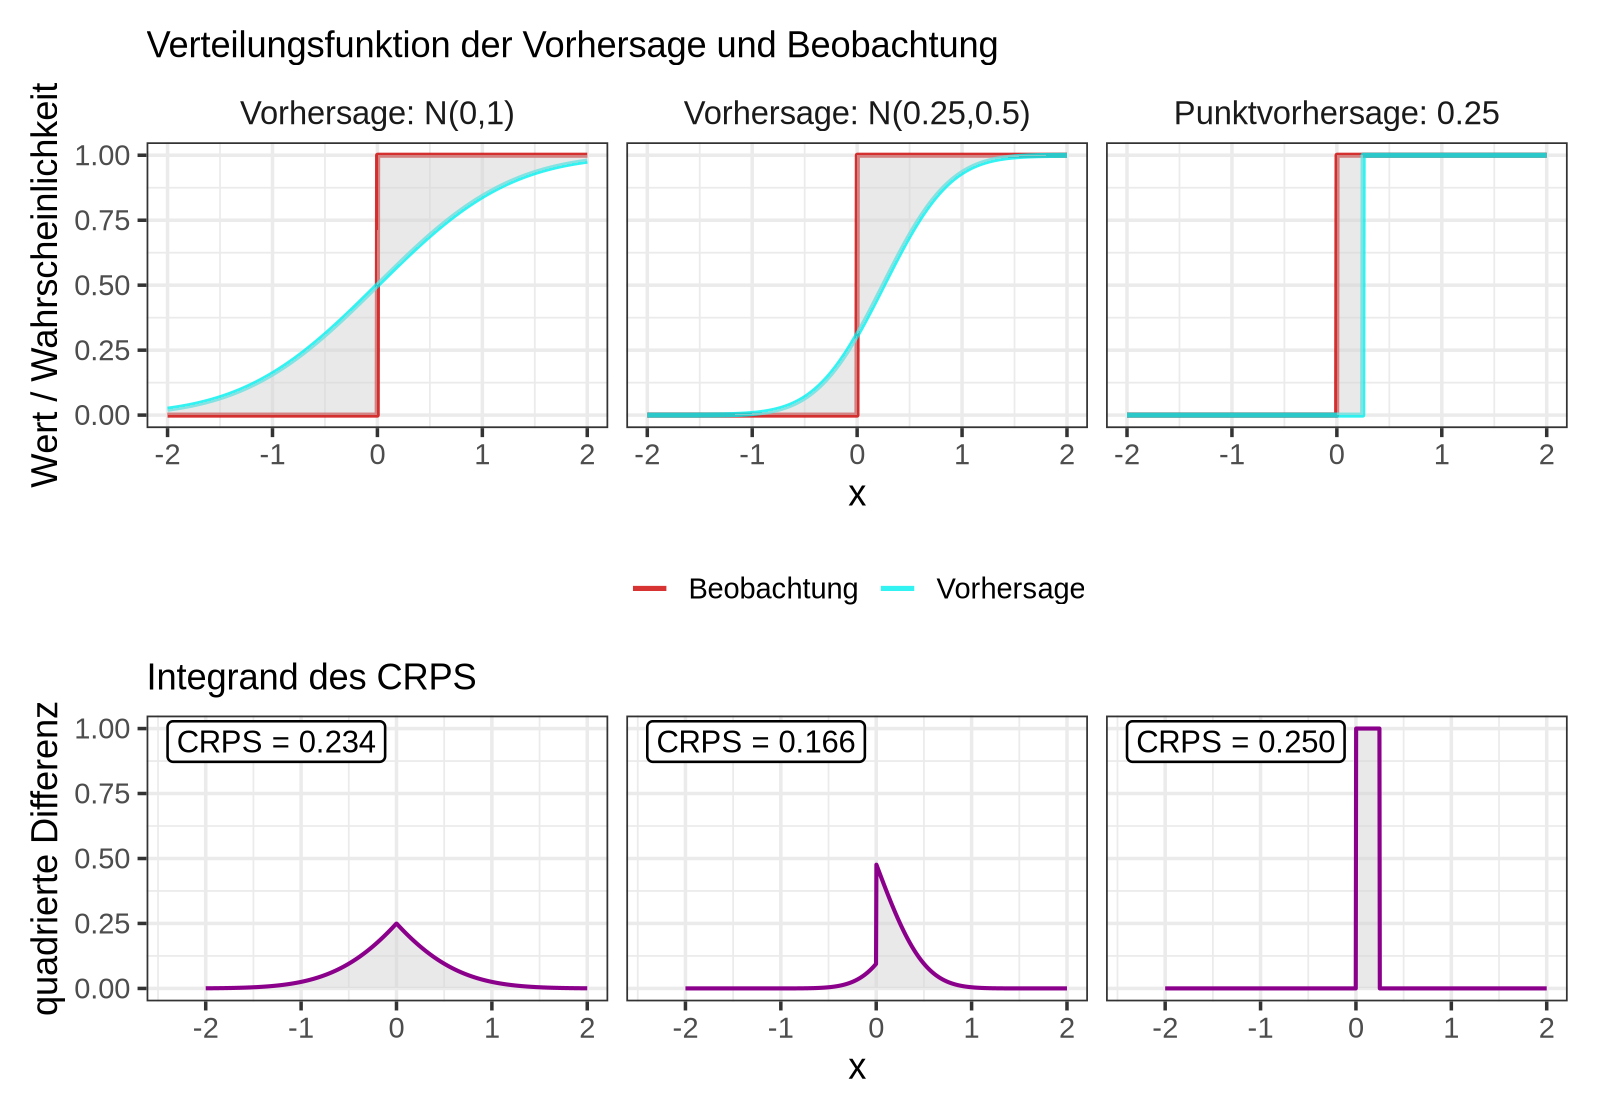
\includegraphics[width=\linewidth]{figs/crps_visu_Rplot.png}
    \caption{CRPS Visualisierung für verschiedene Vorhersagen. Oben wird die Vorhersageverteilungsfunktion mit einer Beobachtung von Wert 0 verglichen. Die Beobachtung ist als Indikatorfunktion dargestellt. Die graue Fläche markiert die Abweichung zwischen beiden Funktionen. Unten ist diese Abweichung für jeden Wert von x quadriert dargestellt. Das Integral über diese quadrierte Differenz ergibt den CRPS.}
    \label{fig:crps_visu}
\end{figure}


Er besitzt mehrere Eigenschaften, die ihn für die Bewertung probabilistischer Vorhersagen attraktiv machen. Erstens benötigen wir, dadurch dass er auf Verteilungsfunktionen basiert, zur Anwendung keine Kenntnisse über die zugehörige Dichtefunktion, was in einigen Anwendungen hilfreich seien kann. Zum anderen reduziert er sich im Fall einer Punktvorhersage (dargestellt als Punktmaß) auf den absoluten Fehler $\abs{x-y}$  \parencite{Gneiting2007}, wie auch in Abbildung \ref{fig:crps_visu} erkennbar ist. Dadurch ist er eine natürliche Verallgemeinerung klassischer Fehlermaße und ermöglicht somit einen direkten Vergleich zwischen Punktvorhersage und probabilistischer Vorhersage. Schließlich liegt der CRPS in derselben Einheit wie die vorhergesagte Größe vor, was seine Interpretation erleichtert.

Den empirischen Gesamtscore bestimmen wir analog zum Quantilscore für Paare der Form \eqref{eq:stich} als
\[
\widehat{\mathrm{CRPS}} = \frac{1}{n}\sum_{i=1}^{n}\CRPS(F_i,y_i).
\]
Um den CRPS zu berechnen, können wir je nach Verteilung, numerische Methoden oder analytische Formen verwenden. Im Allgemeinen sind keine geschlossenen analytischen Ausdrücke verfügbar. Für eine Vielzahl von Verteilungen gibt es diese jedoch \parencite{scoringRules}. Zur Bestimmung solcher Ausdrücke kann folgende alternative Darstellung des CRPS hilfreich sein \parencite{Gneiting2007}: 
\[
\CRPS(F,y)=\mathbb{E}\abs{X-y}-\frac{1}{2}\E\abs{X-X'},\qquad X,X' \overset{\text{i.i.d.}}{\sim} F.
\]
Mit ihr ergibt sich beispielsweise für eine empirische Verteilungsfunktion $F_m$, erzeugt aus Werten $z_1,\dotsc, z_m$ der CRPS als \parencite{scoringRules}
\begin{equation} \label{eq:crps_emp}
\CRPS(F_m,y)= \frac{1}{m}\sum_{i=1}^m\abs{z_i-y}-\frac{1}{2m^2} \sum_{i=1}^m\sum_{j=1}^m\abs{z_i-z_j}.
\end{equation} Für eine Normalverteilung erhaltenen wir
\[
\CRPS\bigl(\mathcal{N}(\mu,\sigma^2), x\bigr)
=
\sigma
\left[
z\left(2\Phi(z)-1\right)
+2\varphi(z)
-\frac{1}{\sqrt{\pi}}
\right]
\quad  \text{mit} \quad
z=\frac{x-\mu}{\sigma},
\]
wobei $\varphi$ die Dichte und $\Phi$ die Verteilungsfunktion der Standardnormalverteilung bezeichnen \parencite{gneiting2014probabilistic}. 


Abschließen führen wir eine weitere Darstellung des CRPS ein, mit der wir einen direkten Bezug zum Quantilscore herstellen. Sie stammt von \textcite{TameaQSCRPS} und lautet
\begin{equation} \label{eq:crps_qs}
\CRPS(F,y)=2\int_0^1 \QS_\alpha(q_\alpha(F),y)\,d\alpha.    
\end{equation}

Der CRPS lässt sich somit als Integral des Quantilscores über alle Quantilniveaus interpretieren. Daraus können wir ein einfache Approzimation des CRPS durch diskretisieren des Integrals an einer endlichen Menge von Quantilen erhalten. Diese Approzimation ist äquivalent zu einer weiteren proper Scoring-Rule dem \emph{Weighted Interval Score}, der probabilistische Vorhersagen anhand mehrerer symmetrisch um den Median gewählter Quantile bewertet \parencite{FakoorQSCRPS}.

Außerdem ermöglicht die Darstellung des CRPS als Quantilscore eine effiziente Berechnung für empirische Verteilungsfunktionen. Für eine empirische Verteilungsfunktion $F_m$ erzeugt aus Werten $z_1 \le \dotsc \le z_m$ können wir den $\CRPS$ folgendermaßen darstellen
\begin{equation} \label{eq:crps_qs_emp}  
\CRPS(F_m,y)=\frac{2}{m}\sum_{k=1}^m (\mathds{1}\{y \le z_k\}-\alpha_k) (z_k-y) \quad \text{mit} \quad \alpha_k=\frac{2k-1}{2m}.
\end{equation} Diese Berechnungsvorschrifft wird beispielsweise standardmäßig im R-Paket \texttt{scoringRules} genutzt \parencite{scoringRules}.




Zusätzlich erhalten wir mit der Darstellung des CRPS über den Quantilscore eine Möglichkeit, ihn besser zu untersuchen, indem wir den verdoppelten erwarteten Quantil\-score in Ab\-hängig\-keit vom Quantil\-niveau darstellen. Die Fläche unter der Kurve entspricht dabei dem erwarteten CRPS, sodass wir erkennen können, welche Quantilbereiche zu dessen Wert beitragen. Beim Vergleich mehrerer Vorhersagen ist eine Vorhersage in einem Quantilbereich besser, wenn ihre Quantilscorekurve unter derjenigen der anderen Vorhersage liegt. Typischerweise erhalten wir einen umgekehrt U-förmigen Verlauf, sodass die mittleren Quantilscores den größten Beitrag zum CRPS leisten, während die Randquantile geringere Scores aufweisen. Eine ähnliche Darstellung verwenden \textcite{Gneiting2007} in Fig. 10, in der der Brier Score (eine konsistente Scoring-Function) in Abhängigkeit vom Schwellenwert dargestellt wird. Sie bezeichnen diese Abbildung als \emph{Prediction-Error-Curve}. In Anlehnung daran bezeichnen wir unsere Darstellung des Quantilscores als \emph{Quantile-Error-Curve}.

\begin{bsp}[Quantile-Error-Curve] \label{bsp:quantile-error-curve}
Wir stellen die Quantile-Error-Curve für den Vorhersagegenstand aus Beispiel \ref{bsp:auto_kal} hinsichtlich der Vorhersagen $F_1,F_2,F_3$ (die ideale, marginale und unfokussierte Vorhersage) aus den Beispielen \ref{bsp:auto_kal} und \ref{bsp:quant_cal} dar.

Abbildung \ref{fig:quantile-error-curve} zeigt die Quantile-Error-Curve der Vorhersagen auf Basis einer Simulation mit $3000$ Stichproben. Wir erkennen einen umgekehrt U-förmigen Verlauf der Quantilscorefunktionen. Dabei ist die Kurve der idealen Vorhersage am niedrigsten in allen Quantilbereichen und weist daher den niedrigsten CRPS auf. Für die marginale und die unfokussierte Vorhersage zeigen sich nahezu identische Kurven, wobei die marginale Vorhersage im mittleren Quantilbereich minimal besser und im äußeren Quantilbereich minimal schlechter ist. Hinsichtlich des CRPS bedeutet das, dass beide Vorhersagen einen ähnlichen Wert haben.
\end{bsp}

\begin{figure}
    \centering
    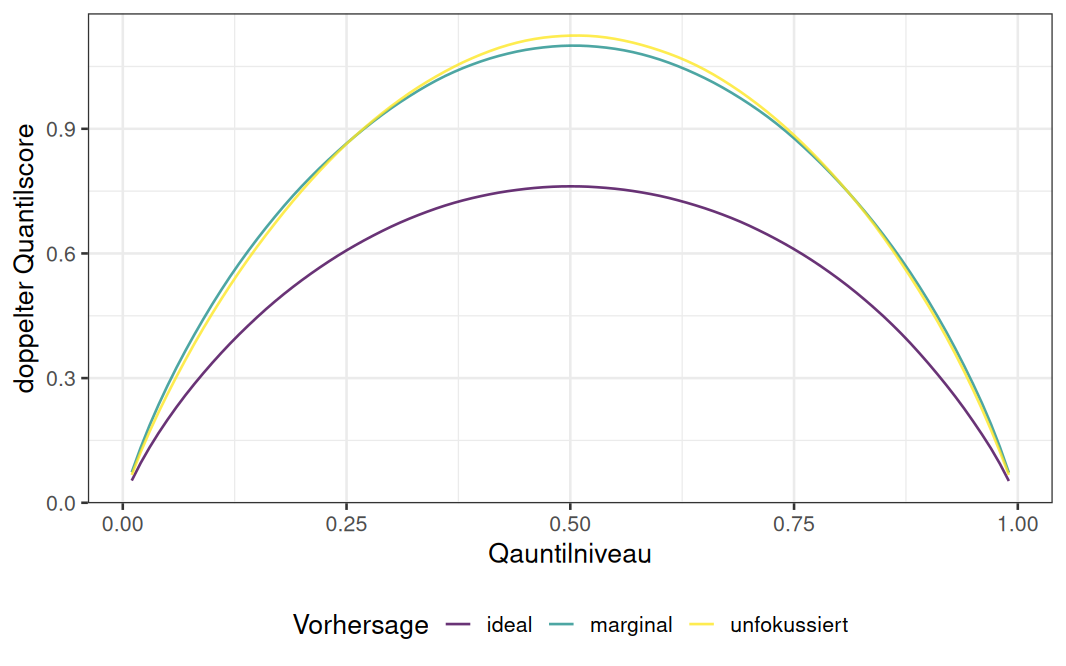
\includegraphics[width=.8\linewidth]{figs/qs_crps_visu_Rplot.png}
    \caption{Quantile-Error-Curve für Beispiel \ref{bsp:quantile-error-curve}
    }
    \label{fig:quantile-error-curve}
\end{figure}{}

Schließlich ist die Darstellung des CRPS über den Quantilscore besonders hilfreich, wenn wir im Folgenden den CRPS in verschiedene Komponenten zerlegen. 





\chapter{Score Zerlegung}  \label{chap:score_decomp}
Wie im vorherigen Kapitel beschrieben ist ein Vorteil von Scores, dass wir mit ihnen eine Vorhersage anhand einer einzigen Zahl bewerten können, was leicht einen Vergleich verschiedener Vorhersagen ermöglicht. Gleichzeitig bleibt zunächst unklar, auf welche Eigenschaften einer Vorhersage der jeweilige Score tatsächlich zurückzuführen ist. Denn Scores berücksichtigen sowohl die Kalibrierung als auch die Schärfe einer Vorhersage \parencite{gneiting2014probabilistic}. Ein guter Score kann daher sowohl aus einer guten Kalibrierung als auch aus einer hohen Schärfe resultieren. Umgekehrt kann ein schlechter Score aus Defiziten in einem oder beiden dieser Aspekte entstehen.

Aus diesem Grund ist es sinnvoll, Scores in einzelne Komponenten zu zerlegen, die Kalibrierung und Schärfe getrennt erfassen. Das ermöglicht eine differenziertere Analyse der Vorhersagequalität und macht transparent, welche Aspekte einer Vorhersage zu ihrem Score beitragen. Entsprechend können Anwender diejenige Vorhersage wählen, die am besten zu ihren Ansprüchen passt. Beispielsweise kann in Anwendungen, in denen verlässliche Wahrscheinlichkeitsaussagen im Vordergrund stehen, eine gut kalibrierte Vorhersage bevorzugt werden, selbst wenn diese geringere Schärfe oder sogar einen insgesamt schlechteren Score als Alternativen aufweist.

In diesem Kapitel geht es daher primär um die Zerlegung des Quantilscores und des CRPS gemäß \textcite{gneiting2023regression} und \textcite{arnold2024decompositions}. In Abschnitt \ref{seq:score_components} beschreiben wir zunächst allgemein die Komponenten und die Idee hinter der Zerlegung, bevor wir sie in Abschnitt \ref{seq:decomp_qs} anhand der Zerlegung des Quantilscores verdeutlichen.  Für die empirische Umsetzung greifen wir auf den in Abschnitt \ref{sec:emp_prüf_quantcal} vorgestellten CORP-Ansatz zur Quantilkalibrierung zurück. Aufbauend auf dieser Zerlegung erläutern wir in Abschnitt \ref{seq:decomp_crps} eine Zerlegung des CRPS, wobei der Fokus auf der empirischen Umsetzung liegt. Anschließend stellen wir in Abschnitt \ref{seq:decomp_visu} eine Möglichkeit zur Visualisierung der Zerlegungen und in Abschnitt \ref{seq:decomp_skill} mit dem Skill Score eine Möglichkeit zur relativen Einordnung von Scores vor. Abschließend beschreiben wir in Abschnitt \ref{seq:decomp_prop} Eigenschaften, die wir uns von Scorezerlegungen wünschen könnem, und dass die in dieser Arbeit verwendeten Zerlegungen des Quantilscores und des CRPS diese Eigenschaften erfüllen.

\section{Komponenten der Zerlegung} \label{seq:score_components}
Gemäß \textcite{gneiting2023regression} erfolgt die Zerlegung eines Scores in drei Komponenten: Unsicherheit, Diskriminationsfähigkeit und Misskalibrierung. Die Unsicherheit (UNC) beschreibt die inhärente Variabilität des Vorhersagegegenstands. Sie ist damit keine Eigenschaft der Vorhersage und kann daher nicht durch Verbesserung dieser reduziert werden. Je höher der Wert, desto größer die Variabilität des Vorhersagegegenstands. Die Diskriminationsfähigkeit (DSC) bezeichnet die Fähigkeit einer Vorhersage, unterschiedliche Situationen zu unterscheiden. Sie entspricht dem Informationsgehalt der Vorhersage und erfasst damit die Schärfe der Vorhersage. Je größer der Wert, desto besser ist die Diskriminationsfähigkeit einer Vorhersage. Die Misskalibrierung (MCB) misst fehlende Kalibrierung. Ein hoher Wert deutet auf schlechte Kalibrierung hin. Für einen erwarteten Score $\bar S$ erhalten wir die Zerlegung
\[
\bar S = \MCB - \DSC + \UNC.
\]

Nun stellt sich die Frage, wie sich diese Komponenten bestimmen lassen. Grundlegend vergleichen wir hierzu den erwarteten Score der ursprünglichen Vorhersage mit den Scores einer marginalen und einer rekalibrierten Referenzvorhersage. Während die marginale Referenzvorhersage auf der marginalen Verteilung des Vorhersagegegenstandes basiert, basiert die rekalibrierte Referenzvorhersage auf dessen bedingter Verteilung gegeben die ursprüngliche Vorhersage. Das Vorgehen wird im Folgenden zunächst am Beispiel der Quantilscorezerlegung verdeutlicht.

\section{Zerlegung des Quantilscores} \label{seq:decomp_qs}
Wir beschreiben die Zerlegung des Quantilscores nach \textcite{gneiting2023regression}. Wie für $\alpha$-Quantilkalibrierung betrachten wir für ein $\alpha \in (0,1)$ das Paar \eqref{eq:qaunt_stich_pop} sowie Vorhersage-Beobachtungspaare der Gestalt \eqref{eq:qaunt_stich_emp}. Zusätzlich führen wir die zur Zerlegung benötigten Referenzvorhersagen ein. Mit 
\[
x_0 \coloneqq q_\alpha(Y)
\] 
bezeichnen wir das marginale $\alpha$-Quantil des Vorhersagegegenstandes $Y$, welches die marginale Referenzvorhersage darstellt.
Wir bezeichnen mit
\[
X_{\mathrm{rc}} \coloneqq q_\alpha(Y \mid q_\alpha(F))
\]
die rekalibrierte Quantilvorhersage. $X_\rc$ gibt also an, wie das vorhergesagte Quantil angepasst werden müsste, damit es, bedingt auf jenes, das tatsächliche Quantil von $Y$ korrekt trifft. Entsprechend gilt, sofern $X=X_\rc$ fast sicher ist, dass die Vorhersage bedingt $\alpha$-quantilkalibriert entsprechend der Gleichung \eqref{eq:cond_alpha_quant_cal} ist. Umgekehrt deuten Abweichungen zwischen diesen Größen auf Defizite in der Kalibrierung hin.

%Im Rahmen des Vorhersageraums sind $X$ und $X_{\mathrm{rc}}$ im Allgemeinen Zufallsvariablen, während $x_0$ eine deterministische Größe ist.
Damit haben wir nun folgende drei Vorhersagen: Die eigentlichen Quantilvorhersagen $X$, die rekalibrierte Quantilvorhersage $X_\rc$ sowie die marginale Referenzvorhersage $x_0$. Für diese bestimmen wir nun die erwarteten Scores gemäß Definition \ref{def:exp_score} und nennen diese den (erwarteten) Gesamtscore $\overline{\QS}_\alpha$, den rekalibrierten Score $\overline{\QS}^{\rc}_\alpha$ und den marginalen Score $\overline{\QS}^{\mg}_\alpha$. Sie lauten also
\[
\overline{\QS}_\alpha \coloneqq \E_\PW[\QS_\alpha(X,Y)], \quad
\overline{\QS}^{\rc}_\alpha \coloneqq \E_\PW[\QS_\alpha(X_{\rc},Y)], \quad
\overline{\QS}^{\mg}_\alpha \coloneqq \E_\PW[\QS_\alpha(x_0,Y)].
\]
Mit diesen Scores können wir nun die Zerlegungskomponenten bestimmen. Sie sind definiert als
\[
\MCB_\alpha \coloneqq \overline{\QS}_\alpha - \overline{\QS}^{\rc}_\alpha, \quad
\DSC_\alpha \coloneqq \overline{\QS}^{\mg}_\alpha - \overline{\QS}^{\rc}_\alpha, \quad
\UNC_\alpha \coloneqq \overline{\QS}^{\mg}_\alpha.
\]
Diese Definitionen spiegeln direkt die inhaltliche Interpretation der drei Komponenten wider: Die Misskalibrierung entspricht der Verbesserung der Vorhersage durch Rekalibrierung, die Diskriminationsfähigkeit den zusätzlichen Informationsgehalt der rekalibrierten gegenüber der marginalen Referenz und die Unsicherheit dem erwarteten Score der marginalen Referenzvorhersage.
Damit haben wir die Zerlegung
\[
\overline{\QS}_\alpha = \MCB_\alpha - \DSC_\alpha + \UNC_\alpha
\]
erhalten.

Auf empirischer Ebene besteht die Herausforderung darin, die rekalibrierten 
Werte $X_{\mathrm{rc}}$ zu bestimmen. Der in Abschnitt \ref{sec:emp_prüf_quantcal} beschriebene 
CORP-Ansatz liefert solche Schätzer mittels des PAV-Algorithmus. Konkret setzen 
wir
\[
\hat{x}_i = \hat{q}_\alpha(Y \mid X = x_i)
\quad \text{und} \quad
\hat{x}_0 = \hat{q}_\alpha(Y),
\]
wobei $\hat{q}_\alpha(Y)$ das empirische $\alpha$-Quantil der Beobachtungen 
und $\hat{x}_i$ die rekalibrierten Qauntile des CORP-Ansatzes bezeichnet. Die empirischen Scores sind dann gegeben durch
\begin{equation} \label{eq:decomp_qs_emp_scores}
\widehat{\QS}_\alpha \coloneqq \frac{1}{n}\sum_{i=1}^{n}\QS_\alpha(x_i,y_i), \;\;
\widehat{\QS}^{\rc}_\alpha \coloneqq \frac{1}{n}\sum_{i=1}^{n}\QS_\alpha(\hat{x}_i,y_i), \;\;
\widehat{\QS}^{\mg}_\alpha \coloneqq \frac{1}{n}\sum_{i=1}^{n}\QS_\alpha(\hat{x}_0,y_i),
\end{equation}
sodass die empirische Zerlegung
\[
\widehat{\QS}_\alpha = \widehat{\MCB}_\alpha - \widehat{\DSC}_\alpha + \widehat{\UNC}_\alpha
\]
mit
\[
\widehat{\MCB}_\alpha \coloneqq \widehat{\QS}_\alpha - \widehat{\QS}^{\rc}_\alpha, \quad
\widehat{\DSC}_\alpha \coloneqq \widehat{\QS}^{\mg}_\alpha - \widehat{\QS}^{\rc}_\alpha, \quad
\widehat{\UNC}_\alpha \coloneqq \widehat{\QS}^{\mg}_\alpha
\]
lautet. 

\section{Zerlegung des CRPS auf Basis des Quantilscores} \label{seq:decomp_crps}
Im Gegensatz zu Scoring-Functions wie dem Quantilscore ist die Zerlegung für Scoring-Rules wie dem CRPS komplizierter. Wieder benötigen wir zur Zerlegung eine marginale und eine rekalibrierte Referenzvorhersage. Im Gegensatz zum Quantilscore handelt es sich bei diesen Referenzvorhersagen jedoch nicht mehr nur um Punktvorhersagen, sondern um probabilistische Vorhersagen. Zudem ist die rekalibrierte Referenzvorhersage stets an einen bestimmten Kalibrierungsbegriff gebunden. Bei der Zerlegung des Quantilscores für das $\alpha$-Quantil ergab sich hierfür die (bedingte) $\alpha$-Quantilkalibrierung als natürliche Bedingung. Für den CRPS wäre daher eigentlich, weil wir mit ihm gesamte Vorhersageverteilungen bewerten, die Auto-Kalibrierung der natürliche Kalibrierungsbegriff. In diesem Fall lautete die marginale Referenzvorhersage
\begin{equation}\label{eq:marg_ref_crps}
    F_0 \coloneqq \LW(Y)
\end{equation}
und die rekalibrierte Referenzvorhersage 
\[
F_\rc\coloneqq \LW \left(Y \mid F \right).
\] 
Eine Zerlegung des CRPS hinsichtlich der Auto-Kalibrierung erweist sich jedoch empirisch als wenig geeignet (Begründung in Abschnitt \ref{seq:decomp_prop}). Alternativ kann der CRPS auch hinsichtlich anderer Kalibrierungsbegriffe zerlegt werden. Hierfür lassen sich äquivalente Darstellungen des CRPS verwenden. Eine Möglichkeit ist die Zerlegung hinsichtlich Quantilkalibrierung (Definition \ref{def:all_quantcal}) für die wir die Darstellung des CRPS über den Quantilscore \eqref{eq:crps_qs} verwenden können. 
Diese Zelegung gemäß \textcite{arnold2024decompositions} wird im Folgenden aufgeführt. Im Gegensatz zur Quantilscorezerlegung beschränken wir uns hier auf die empirische Umsetzung, weil wir die entsprechenden Populationsterme analog konstruieren können.

Die Grundidee besteht darin, dass wir durch die Darstellung des CRPS als Integral der Quantilscores \eqref{eq:crps_qs} die Rekalibrierung auf die Ebene der einzelnen Quantile verlagern können. Somit umgehen wir zugleich die direkte Konstruktion probabilistischen Referenzvorhersagen. Stattdessen führen wir die bereits für den Quantilscore entwickelte Zerlegung für mehrere Quantile separat durch und übertragen sie anschließend auf den CRPS. 


%Somit umgehen wir zugleich die direkte Konstruktion probabilistischen Referenzvorhersagen und ¨ubertragendie Zerlegung des Quantilscores ¨uber die Quantildarstellung auf den CRPS direkt
Für Vorhersage-Beobachtungspaare der Form \eqref{eq:stich} schreiben wir mit \eqref{eq:crps_qs} und \eqref{eq:decomp_qs_emp_scores} den empirischen Gesamtscore als
\begin{equation}\label{eq:decomp_crps}
    \widehat{\CRPS}= \frac{1}{n}\sum_{i=1}^{n} 2\!\int_0^1 \QS_\alpha(q_\alpha(F_i),y_i)\,d\alpha = 2 \int_0^1\widehat{\QS}_\alpha \,d\alpha.
\end{equation} 
Aufgrund dieser Darstellung können wir den marginalen und den rekalibrierten Score analog aus den entsprechenden Quantilscores konstruieren:
\begin{equation} \label{eq:decomp_crps_scores}
  \widehat{\CRPS}^{\rc}=2 \int_0^1\widehat{\QS}^{\rc}_\alpha \,d\alpha, \quad \quad
  \widehat{\CRPS}^{\mg}=2 \int_0^1\widehat{\QS}^{\mg}_\alpha \,d\alpha .
\end{equation}
Für den rekalibrierten Score nutzen wir also die durch den CORP-Ansatz bestimmten rekalibrierten bedingten Quantile als Vorhersagen und für den marginalen Score die Quantile der Beobachtungen als Vorhersagen. So erlangen wir
\[
\widehat{\CRPS} = \widehat{\MCB} - \widehat{\DSC} + \widehat{\UNC}\\
\]
mit
\[
\widehat{\MCB}=\widehat{\CRPS} - \widehat{\CRPS}^{\rc}, \quad
\widehat{\DSC}=\widehat{\CRPS}^{\mg} - \widehat{\CRPS}^{\rc}, \quad
\widehat{\UNC}= \widehat{\CRPS}^{\mg}\;
\]

Zur Berechnung der verschiedenen Scores \eqref{eq:decomp_crps} und \eqref{eq:decomp_crps_scores} müssen Integrale gelößt werden. Diese approximieren wir numerisch. Dazu verwenden wir in der vorliegenden Arbeit die Gauß-Legendre-Quadratur \parencite{gautschi2004orthogonal} mit 25 Stützstellen auf dem Intervall $[0,1]$. Bezeichnen $(\alpha_k,w_k)^{25}_{k=1}$ die zugehörigen Stützstellen und Gewichte, so approximieren wir
\begin{align}
    \widehat{\CRPS}& = 2\int_0^1\widehat{\QS}_\alpha \,d\alpha \approx 2 \sum_{k=1}^{25}w_k\, \widehat{\QS}_{\alpha_k}  \\
    \widehat{\CRPS}^{\rc}&=2 \int_0^1\widehat{\QS}^{\rc}_\alpha \,d\alpha \approx 2 \sum_{k=1}^{25}w_k\, \widehat{\QS}^{\rc}_{\alpha_k}
\end{align}
Für den erwarteten rekalibrierten Score bestimmen wir also für alle Stützstellen $\alpha_k$ die rekalibrierten Quantile mithilfe des CORP-Ansatzes.

Für empirische Vorhersageverteilungen erfolgt die Berechnung des CRPS hingegen direkt über die Darstellung \eqref{eq:crps_qs_emp}, sodass keine numerische Quadratur erforderlich ist. Für den erwarteten rekalibrierten Score bestimmen wir dann die rekalibrierten Quantile für die Niveaus
\[
\alpha_k=\frac{2k-1}{2m},\qquad k=1,\dots,m,
\]
wobei $m$ die Anzahl der Werte der empirischen Vorhersageverteilung bezeichnet.



Aufgrund der unterschiedlichen Berechnungsmethoden können beim Vergleich von Vorhersagen auf Basis empirischer Vorhersageverteilungen mit Vorhersagen auf Basis stetiger Verteilungsfunktionen numerische Abweichungen im marginalen Score auftreten. Das ist insofern problematisch, da der marginale Score die Unsicherheitskomponente der Zerlegung bestimmt, die ausschließlich auf dem Vorhersagegegenstand beruht und somit für alle Vorhersagen identisch sein sollte. Um solche numerischen Abweichungen zu vermeiden, verwenden wir daher eine einheitliche alternative Berechnungsmethode für den marginalen Score bzw. die Unsicherheitskomponente. Die folgende Aussage liefert die Grundlage für diese Berechnung.

\begin{theo}[Marginaler Score der CRPS-Quantilscorezerlegung entpricht marginalem Score der Zerlegung bzgl. Autokalibrierung \texorpdfstring{\parencite[Proposition 2.2]{arnold2024decompositions}})] \label{theo:crps_mg_eqi}
    \[
        \widehat{\CRPS}^{\mg}=2 \int_0^1\widehat{\QS}^{\mg}_\alpha \,d\alpha = \frac{1}{n}\sum_{i=1}^n \CRPS\left(\widehat{\PW}(Y \leq \cdot) ,y_i\right),
    \]
     wobei  $\;\widehat{\PW}(Y \leq \cdot)$ entsprechend \eqref{eq:Y_mg}, die empirische marginale Verteilung des Vorhersagegegenstandes beschreibt und damit die empirische Variante der marginalen Referenzvorhersageverteilung $F_0$ \eqref{eq:marg_ref_crps} darstellt .
\end{theo}
Das heißt, bei der Quantilscorezerlegung entspricht der marginale Score dem mittleren CRPS der empirischen marginalen Verteilung des Vorhersagegegenstandes. Dadurch lässt sich die $\widehat{\UNC}$-Komponente unabhängig von der Berechnungsmethode einheitlich darstellen und effizient berechnen mit:
\begin{align*}
\widehat{\CRPS}^{\mg}&=2 \int_0^1\widehat{\QS}^{\mg}_\alpha \,d\alpha \\
                    &= \frac{1}{n}\sum_{i=1}^n \CRPS\left(\widehat{\PW}(Y \leq \cdot),y_i\right) && ,\text{Theorem \ref{theo:crps_mg_eqi}}\\ %theorem
                    &= \frac{1}{n}\sum_{i=1}^n\left[\frac{1}{n}\sum_{j=1}^n\abs{y_j-y_i}-\frac{1}{2n^2} \sum_{k=1}^n\sum_{j=1} ^n\abs{y_k-y_j}\right] && ,\text{\eqref{eq:crps_emp}}\\ %empirische rgel
                    &= \frac{1}{2n^2}\sum_{k=1}^n\sum_{j=1}^n\abs{y_k-y_j} \\
                    &= \frac{1}{n^2}\sum_{k=1}^n(2k-n-1)\cdot y_k. %hier noch die Rechenvorschrift
\end{align*}
Die letzte Gleichheit folgt aus der Darstellung der Summe absoluter Differenzen für aufsteigend sortierte Beobachtungen, wobei für die Gültigkeit die $y_k$ aufsteigend sortiert sein müssen.











\section{Darstellen der Score Zerlegung} \label{seq:decomp_visu}
%gucken das miskalibrierung mit einem s geschriebnen
Zu visuellen Darstellung einer Score Zerlegung orientieren wir und an \textcite{gneiting2023model} und \textcite{arnold2024decompositions}. Dazu bilden wir auf der x-Achse die Miskalibrierung (MCB) und auf der y-Achse die Diskriminationsfähikeit (DSC) verschiedener Vorhersagen ab. Höhenlinien zeigen gleiche erwartete Scores. Je weiter links ein Punkt liegt, desto besser ist eine Vorhersage kalibriert, je höher eine Vorhersage liegt desto besser ist ihre Diskriminationsleistung. Damit sind die besten Vorhersagen oben links in der Darstellung. Zusätzlich stellen wir die UNC-Komponente im Plot dar, sodass die erwarteten Scores der Vorhersagen direkt mit dem marginalen Referenzscore verglichen werden können. Die Darstellung ermöglicht es insbesondere, mehrere Vorhersagen gleichzeitig hinsichtlich ihrer Score Komponenten zu vergleichen. Dadurch werden die unterschiedlichen Eigenschaften der Vorhersagen unmittelbar zueinander in Beziehung gesetzt. Das folgende Beispiel verdeutlicht die Darstellung.

\begin{figure}[!h]
    \centering
    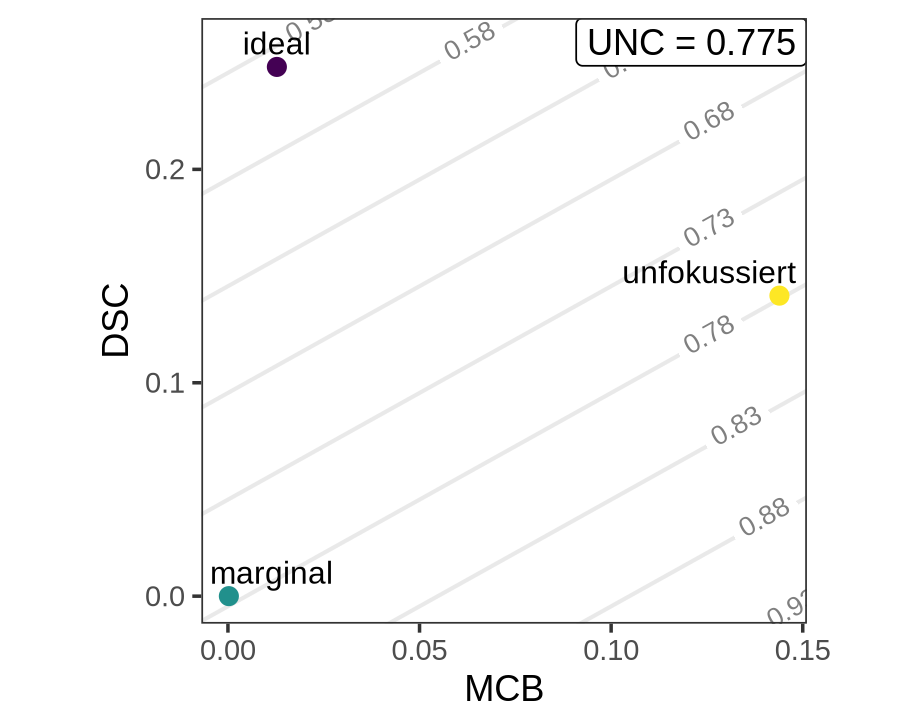
\includegraphics[width=0.55\linewidth]{figs/decomp_visu_Rplot.png}
    \caption{CRPS Zerlegungsdiagramm für das Beispiel \ref{bsp:crps_decomp}.}
    \label{fig:decomp_visu}
\end{figure}

\begin{bsp}[Mehrwert durch Score Zerlegung] \label{bsp:crps_decomp}
Wir zerlegen den CRPS für die Daten und Vorhersagen aus Beispiel \ref{bsp:quantile-error-curve}. Abbildung \ref{fig:decomp_visu} zeigt das CRPS Zerlegungsdiagramm.

Im Diagramm ist die ideale Vorhersage weit oben links zu finden und weist damit sowohl eine hohe Diskriminationsfähigkeit als auch eine geringe Miskalibrierung auf. Die marginale Vorhersage liegt ebenfalls weit links, jedoch ist die Diskriminationsfähigkeit bei null. Die unfokussierte Vorhersage liegt zwischen diesen beiden Vorhersagen: Sie erreicht eine höhere Diskriminationsfähigkeit als die marginale Vorhersage, weist jedoch gleichzeitig eine stärkere Miskalibrierung auf.

Die kaum vorhandene Miskalibrierung der marginalen und der idealen Vorhersage ist darauf zurückzuführen, dass beide auto-kalibriert sind. Die ideale Vorhersage nutzt dabei die vollständige relevante Information über den Vorhersagegegenstand und erreicht daher die höchste Diskriminationsfähigkeit. Die marginale Vorhersage ist hingegen statisch, kann daher nicht zwischen Vorhersagesituationen unterscheiden und weist folglich keine Diskriminationsfähigkeit auf. Die unfokussierte Vorhersage nutzt zwar Information über den latenten Zustand, ist aber durch den zufälligen Regimewechsel schlechter kalibriert, sodass sie insgesamt ähnlich wie die marginale Vorhersage im Gesamtscore abschneidet.

Somit ermöglicht das Diagramm, die unterschiedlichen Eigenschaften der Vorhersagen allein anhand ihrer Position zu erkennen, ohne dass ihre konkrete Konstruktion bekannt sein muss.
\end{bsp}

Eine Einschränkung dieser Darstellung besteht jedoch darin, dass sie stets relativ zu den Vergleichsvorhersagen ist: Die Darstellung kann somit im Sinne eines „Einäugigen unter den Blinden“ eine Vorhersage vergleichsweise gut erscheinen lassen, ohne dass sie tatsächlich eine gute Vorhersage darstellt. Diese relative Bewertung motiviert die Betrachtung des Skill Scores als ergänzendes Maß für die Vorhersagequalität.


\section{Skill Score} \label{seq:decomp_skill}
Absolute Score Werte können schwer einzuordnen sein. Daher ist es hilfreich die Vorhersage zum Score einer Referenz ins Verhältnis zu setzten. Dazu definieren wir den Skill einer Vorhersage als die relative Verbesserung einer Vorhersage gegenüber der marginalen Referenzvorhersage.

\begin{defi}[Skill \parencite{gneiting2023regression}]
Sei $\hat S$ ein empirisch erwarteter Score für eine Vorhersage $F$ und $\hat{S}^\mg$ der erwartete Score einer passenden marginalen Referenzvorhersage, dann heißt
    \[
    \hat S_{\mathrm{skill}}=1-\frac{\hat S}{\hat{S}^\mg}=\frac{\hat{S}^\mg-\hat{S}}{\hat{S}^\mg}=\frac{\widehat{\DSC_S}-\widehat{\MCB_S}}{\widehat{\UNC_S}}
    \]
der Skill der Vorhersage $F$.
\end{defi}

Vor allem ist die letzte Gleichung hinsichtlich der Scorezerlegung interessant. Demnach kann der Skill als Anteil der durch die Vorhersage erklärten Unsicherheit interpretiert werden: Die Diskriminierung beschreibt den Informationsgewinn gegenüber der marginalen Referenzvorhersage, während die Misskalibrierung diesen Gewinn reduziert.

Grundsätzlich kann dieser Wert sowohl positive als auch negative Werte annehmen. Ein positiver Wert bedeutet, dass die Vorhersage besser als die marginale Referenzvorhersage ist, während ein negativer Wert eine schlechtere Vorhersagequalität anzeigt. Werden, wie in dieser Arbeit, Scores mit einem minimalen Wert von null betrachtet, ist der Skill nach oben durch $1$ beschränkt. Üblicherweise ist eine Vorhersage jedoch besser als die marginale Referenz, sodass der Skill im Intervall $[0,1]$ liegt. Insofern können wir den Skill in Analogie als eine Art Determinationskoeffizienten interpretieren \parencite{gneiting2023regression}.


\section{Eigenschaften der Score Zerlegung} \label{seq:decomp_prop}
Als nächstes sollen wünschenswerte Eigenschaften für Score Zerlegung beschreiben werden. Dafür definieren wir zunächst die Score Zerlegung allgemein.

\begin{defi}[Allgemeine Score Zerlegung] \label{def:general_score_decomp}
Sei $\bar S$ der erwartete Score einer Vorhersage $F$. Weiter bezeichnen $\bar S^{\mathrm{rc}}$ den erwarteten Score einer rekalibrierten Version der Vorhersage und $\bar S^{\mathrm{mg}}$ den erwarteten Score einer marginale Referenzvorhersage.
Mit den drei erwarteten Scores können wir die Zerlegung
\[
\bar S = \MCB - \DSC + \UNC
\]
erzeugen mit
\[
\MCB=\bar S - \bar{S}^\rc, \quad
\DSC=\bar{S}^\mg - \bar{S}^\rc, \quad
\UNC= \bar{S}^\mg.
\]
\end{defi}

In Tabelle \ref{tab:vergleich_eigenschaften} sind die Eigenschaften die eine Score Zerlegung erfüllen sollte zusammengefasst. Diese leiten wir aus den auf populations und empirischer Ebene formulierten Eigenschaften der CRPS-Zerlegung von \textcite{arnold2024decompositions} ab.

\begin{table}[htbp]
\caption{Gewünschte Eigenschaften für Score-Zerlegung auf populations- und empirischer Ebene.}
\centering
\fontsize{10}{12}\selectfont

\begin{tabularx}{\textwidth}{@{}p{1.2cm}X p{1.2cm}X@{}}
\hline
\multicolumn{2}{c}{Populationseigenschaften} &
\multicolumn{2}{c}{Empirische Eigenschaften} \\
\hline

P1 & Die Zerlegung ist exakt,
\[
\bar S = \mathrm{MCB} - \mathrm{DSC} + \mathrm{UNC}.
\]
&
E1 & Die Zerlegung ist exakt,
\[
\hat S = \widehat{\mathrm{MCB}}
- \widehat{\mathrm{DSC}}
+ \widehat{\mathrm{UNC}}.
\]
\\[-0.7cm]

P2 & Die Komponenten $\MCB$, $\DSC$ und $\UNC$ sind nichtnegativ.
&
E2 & Die Komponenten $\widehat{\MCB}$,
$\widehat{\DSC}$ und $\widehat{\UNC}$ sind nichtnegativ.
\\[0.4cm]

P3 & Wenn die Vorhersage für einen geeigneten Kalibrierungsbegriff kalibriert ist, gilt $\MCB=0$.
&
E3 & Die Zerlegung ist nicht degeneriert. Eine Zerlegung heißt degeneriert, wenn
$\displaystyle
\hat S = \widehat{\mathrm{MCB}}
$
gilt, falls die Vorhersagen paarweise verschieden sind.
\\[0.3cm]

P4 & $\DSC=0$, wenn die Vorhersage konstant ist.
&
E4 & $\widehat{\DSC}=0$, wenn die Vorhersage konstant ist.
\\[0.3cm]

P5 & Die UNC-Komponente hängt ausschließlich von der marginalen Verteilung des Vorhersagegegenstandes ab.
&
E5 & Die UNC-Komponente kann durch die empirische Verteilung der Beobachtungen
$y_1,\dotsc,y_n$ ausgedrückt werden.
\\[0.3cm]

P0 & Für empirische Maße reduzieren sich die Komponenten $\MCB$, $\DSC$ und $\UNC$ auf die entsprechenden empirischen Komponenten.
&
\multicolumn{2}{l}{} \\

\hline
\end{tabularx}

\label{tab:vergleich_eigenschaften}
\end{table}






%P3 habe ich minimal aufgeweicht damit ich keine großen asumptinos für den quantilscore
Als Nächstes geht es um die Bedeutung der einzelnen Eigenschaften und wie sie miteinander zusammenhängen. Die Eigenschaften P1 und P2 entsprechen in Verbindung mit P0 direkt den empirischen Eigenschaften E1 bzw. E2. Die Eigenschaften P4/E4 und P5/E5 stellen sicher, dass Diskriminationsfähigkeit und Unsicherheit die jeweils gewünschte Interpretation behalten: Eine konstante Vorhersage besitzt keine Diskriminationsfähigkeit, während die Unsicherheit ausschließlich von der Verteilung des Vorhersagegegenstands abhängen soll.

Entscheidend ist die Eigenschaft P3. Für diese muss zunächst ein geeigneter Kalibrierungsbegriff festgelegt werden. Je nachdem welchen wir wählen, müssen die rekalibrierten Vorhersagen, die wir zur Berechnung des rekalibrierten Scores $S^\rc$ benötigen, bezüglich diesem kalibriert sein. 
%Bei der Zerlegung des Quantilscores für das $\alpha$-Quantil ergibt sich hierfür etwa $\alpha$-Quantilkalibrierung als natürlichen Kalibrierungsbegriff. Allgemein gilt für ein einen konsistenten Score, dass wir den Kalibrierungsbegriff wählen bzgl. dessen dieser Score konsistent ist \parencite{gneiting2023regression}.

Nun erläutern wir, dass die in den vorherigen Abschnitten eingeführten Zerlegungen diese Eigenschaften erfüllen. Die Quantilscorezerlegung für ein $\alpha$-Quantil erfüllt Populationseigenschaften P1 bis P5, wobei P3 bezüglich der $\alpha$-Quantilkalibrierung erfüllt ist. Die Eigenschaften folgen direkt aus ihrer Konstruktion, indem wir Theorem 2.23 aus \textcite{gneiting2023regression} auf den Quantilscore anwenden.

Ebenfalls erfüllt die Zerlegung die Eigenschaften E1 bis E5. Dafür ist die Optimalität der durch den PAV-Algorithmus erzeugten rekalibrierten Werte
entscheidend. Diese Eigenschaft soll genauer erläutert werden. Die Grundlage hierfür bildet Theorem 3.1 von \textcite{gneiting2023regression}, dass wir auf den Fall 
des $\alpha$-Quantils spezifizieren.

\begin{theo}[PAV-Algorithmus für Quantile erzeugt optimale rekalibrierte Werte unter Monotonie]
Seien $\hat x_1 \le \dotsc \le \hat x_n$ rekalibrierte Werte erzeugt durch den PAV-Algotihmus für $\alpha$-Quantile \ref{alq:pava}. Diese Folge ist für alle Scoring-Rules $S$, die für das $\alpha$-Quantil unter milden Regularitätsbedingungen konsistent sind (insbesondere dem Quantilscore $\QS_\alpha$) optimal bzgl. der Beobachtungen der From \ref{eq:qaunt_stich_emp} im Sinne von
\[
\frac{1}{n}\sum_{i=1}^n S(\hat{x}_i,y_i) \leq \frac{1}{n}\sum_{i=1}^n S(t_i,y_i)
\]
für jede monoton steigende Folge \(t_1 \leq \dots \leq t_n\).
\end{theo}

Zusammenfassend erfüllt die Zerlegung damit auch die empirischen Eigenschaften E1, E2, E4 
und E5 \parencite[Theorem 3.3, angewendet auf Quantile]{gneiting2023regression}.  Eigenschaft E3 lässt sich anhand eines Beispiels leicht veranschaulichen.

Betrachten wir nun die Eigenschaften der CRPS Zerlegung über den Quantilscore. Eigentlich wäre für den CRPS Auto-Kalibrierung der natürliche Kalibrierungsbegriff. Allerdings stehen P3 und E3 in einem Spannungsverhältnis: Wird P3 bezüglich der Auto-Kalibrierung erfüllt, so wird die empirische Zerlegung des CRPS degeneriert \parencite{arnold2024decompositions}. Das bedeutet, dass im Fall von paarweise verschiedenen Vorhersagen, die gesamte Scoredifferenz der Misskalibrierung zugeschrieben würde, sodass die Zerlegung keinen praktischen Erkenntnisgewinn mehr liefert. Daher mussten wir für eine praktisch sinnvolle und robuste Zerlegung des CRPS auf den schwächeren Kalibrierungsbegriff der Quantilkalibrierung zurückgreifen. 
\textcite{arnold2024decompositions} zeigen, dass diese Zerlegung die empirischen Eigenschaften E1 bis E5 erfüllt (Proposition~2.2) sowie die Populationseigenschaften P0 bis P5 (Theorem~4.4). Dabei wird die Eigenschaft P3 hinsichtlich Quantilkalibrierung erfüllt.

Für eine umfangreiche Übersicht anderer Zerlegungsansätze des CRPS siehe \textcite{arnold2024decompositions}.

%Hierzu gibt es mehrere Möglichkeiten. Da im Rahmen dieser Arbeit neben dem CRPS auch der Quantilscore betrachtet wird, nutzen wir für die Zerlegung des CRPS die Darstellung \eqref{eq:crps_qs}, sodass die beschriebene Zerlegung hinsichtlich Quantilkalibrierung erstellt wird. Für andere Zerlegungsmöglichkeiten des CRPS siehe \textcite{arnold2024decompositions}.

